% !TEX root = /home/fred-olav/afgv/src/preamble.tex
\input preamble.tex

\noindent

\vskip 5pt

\textbf{Læringsoppdrag Reguleringsteknikk - Stasjon 04 }

Dette læringsoppdraget består av følgende:

\begin{itemize}[noitemsep]
	\item Oppgavesett Reguleringsteknikk
	\item Oppgavesett PID-regulatoren
	\item Oppgavesett Kaskadekobletregulering
	\item Oppgavesett Foroverkobletregulering
	\item Arbeidsoppdrag på Stasjon 04 
\end{itemize}

\vskip 5pt 
Du kan jobbe parallelt med alle oppgavene. 
$$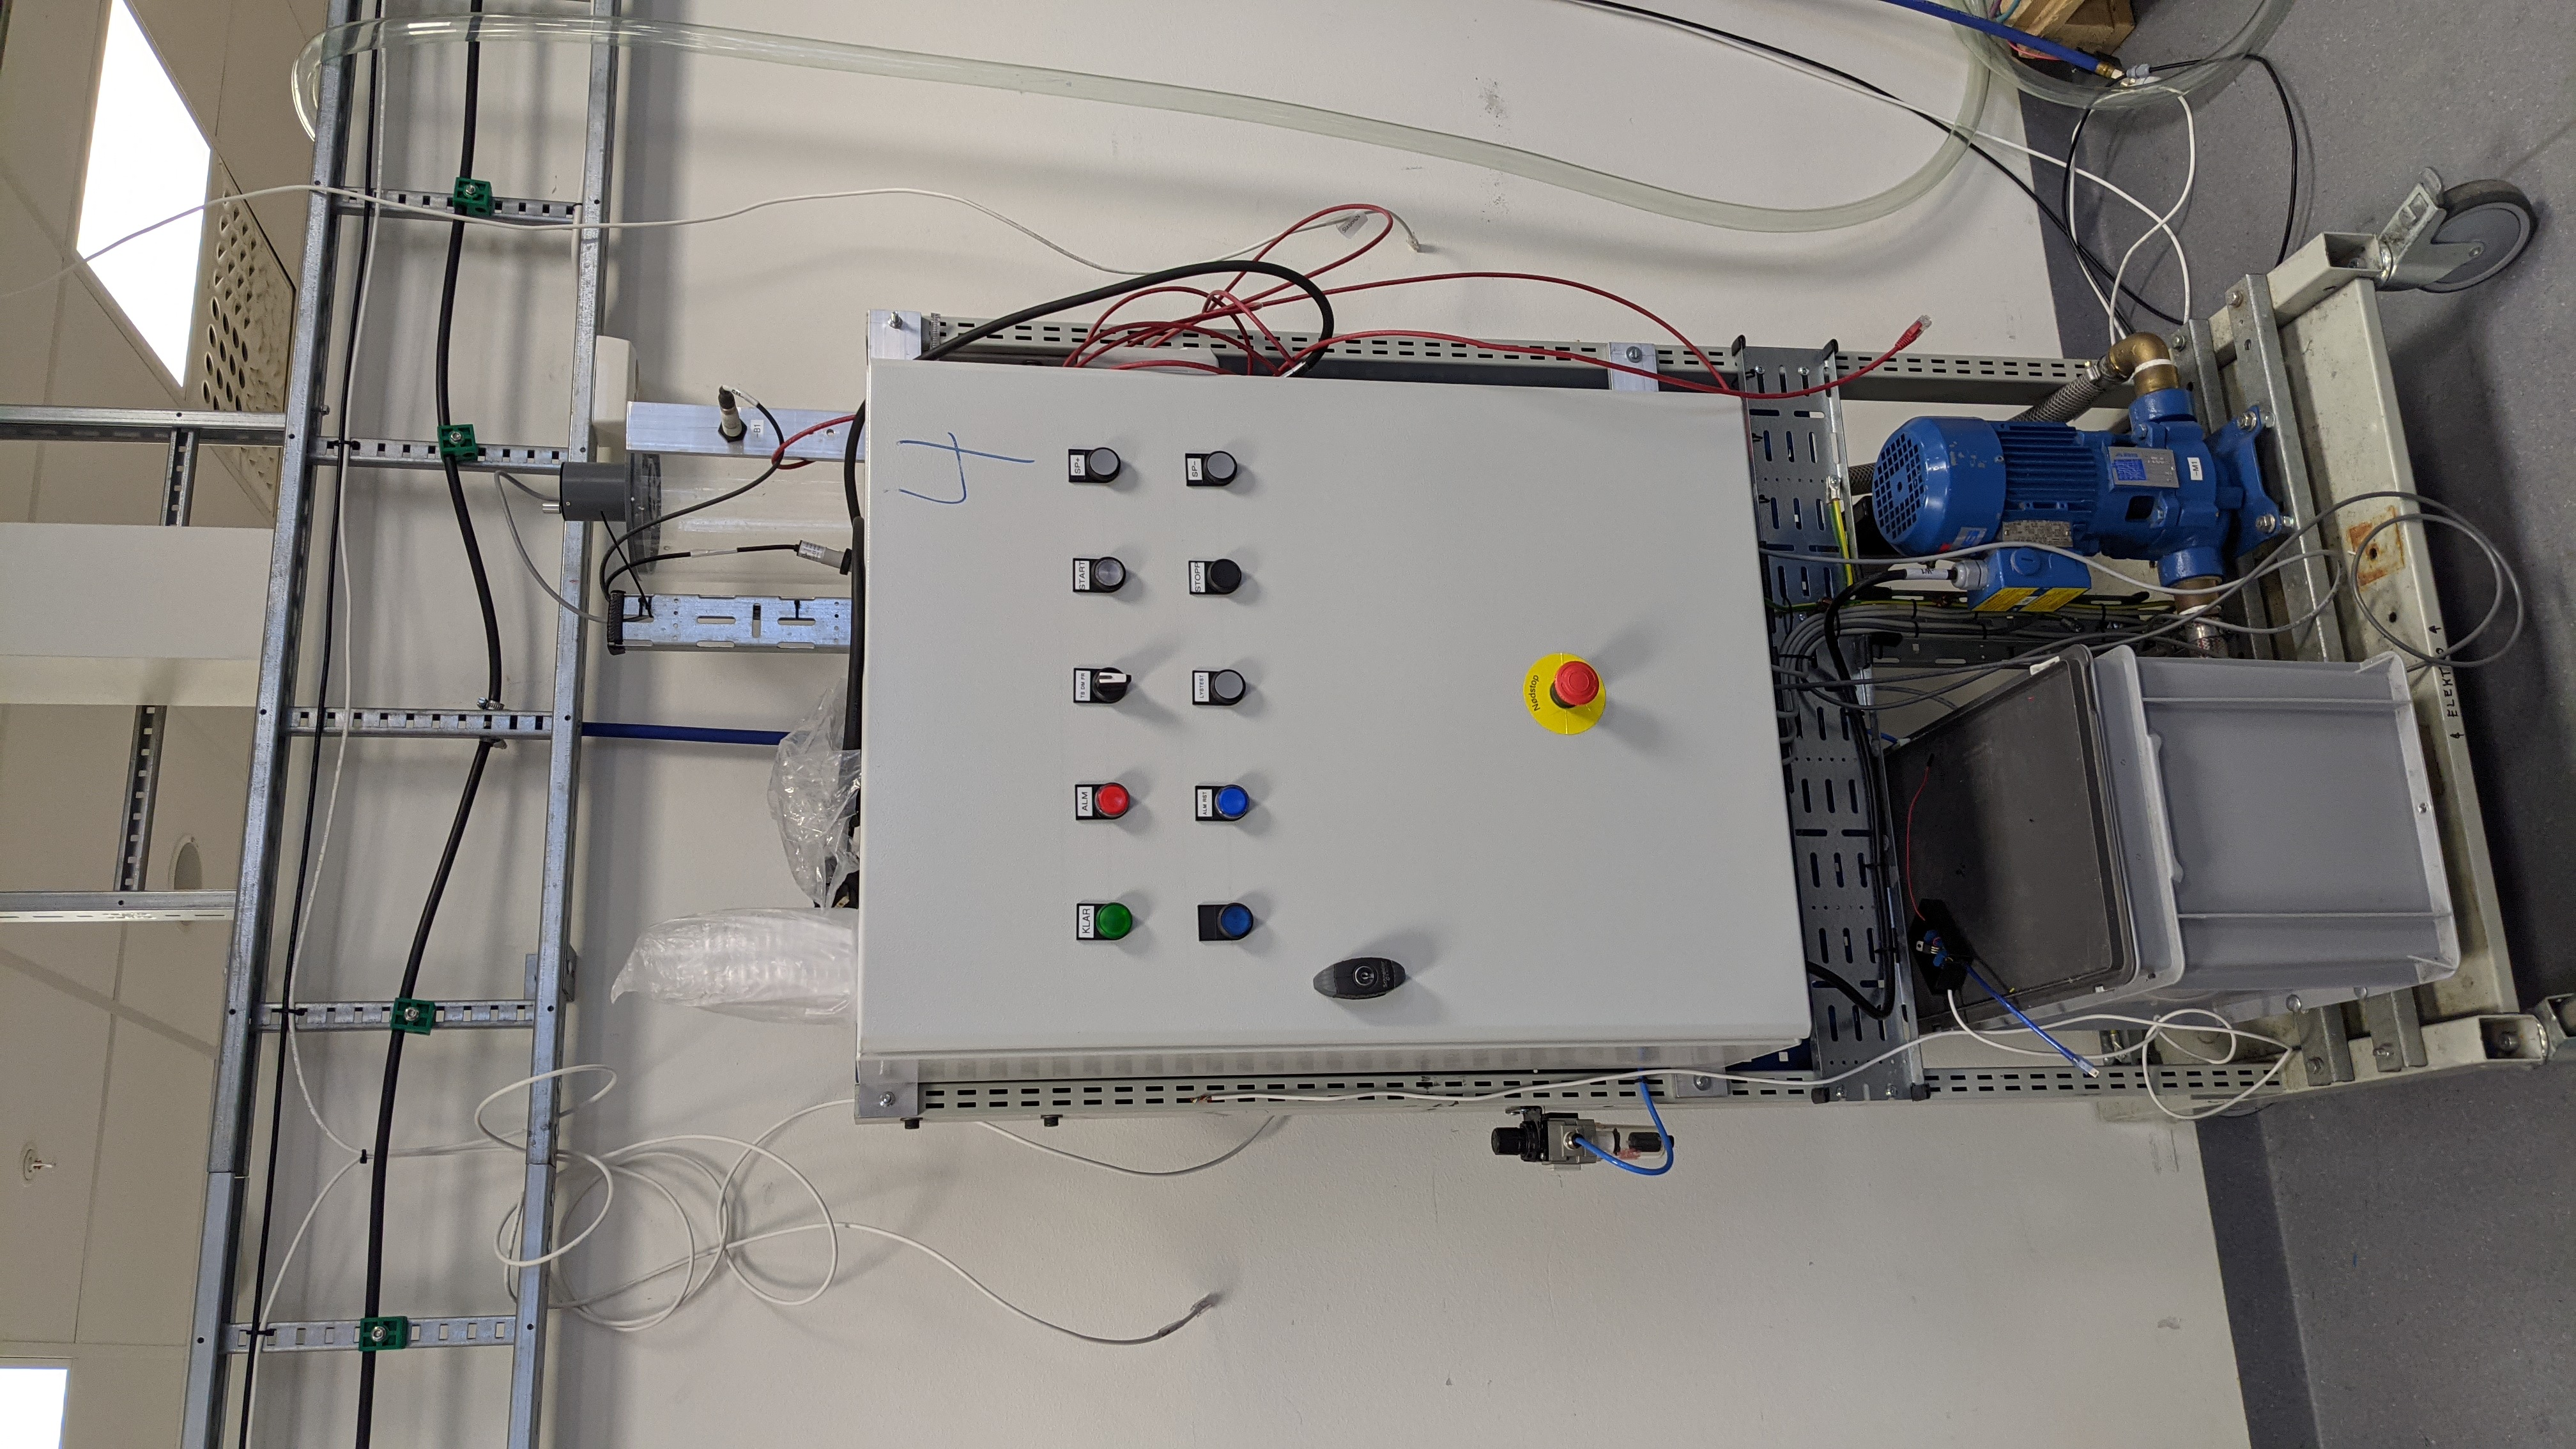
\includegraphics[height=10cm,angle=-90]{./stasjon04x01.jpg}$$\\
\vskip 5pt
\textbf{Bakgrunnsteori}
 I filen \href {https://autofaget.no/pdfs/afgv.pdf}{afgv.pdf} er følgende kapittler til hjelp for dette læringsoppdraget:
 \begin{itemize}[noitemsep]
	 \item Instrument kalibrering
	 \item Continuous pressure measurement
	 \item Kontinuerlig nivåmålig
	 \item Continuous temperature measurement
	 \item Continuous fluid flow measurement
	 \item Control valves
	 \item Closed-loop control
	 \item Process dynamics and PID controller tuning
	 \item Basic process control strategies
 \end{itemize}
%$$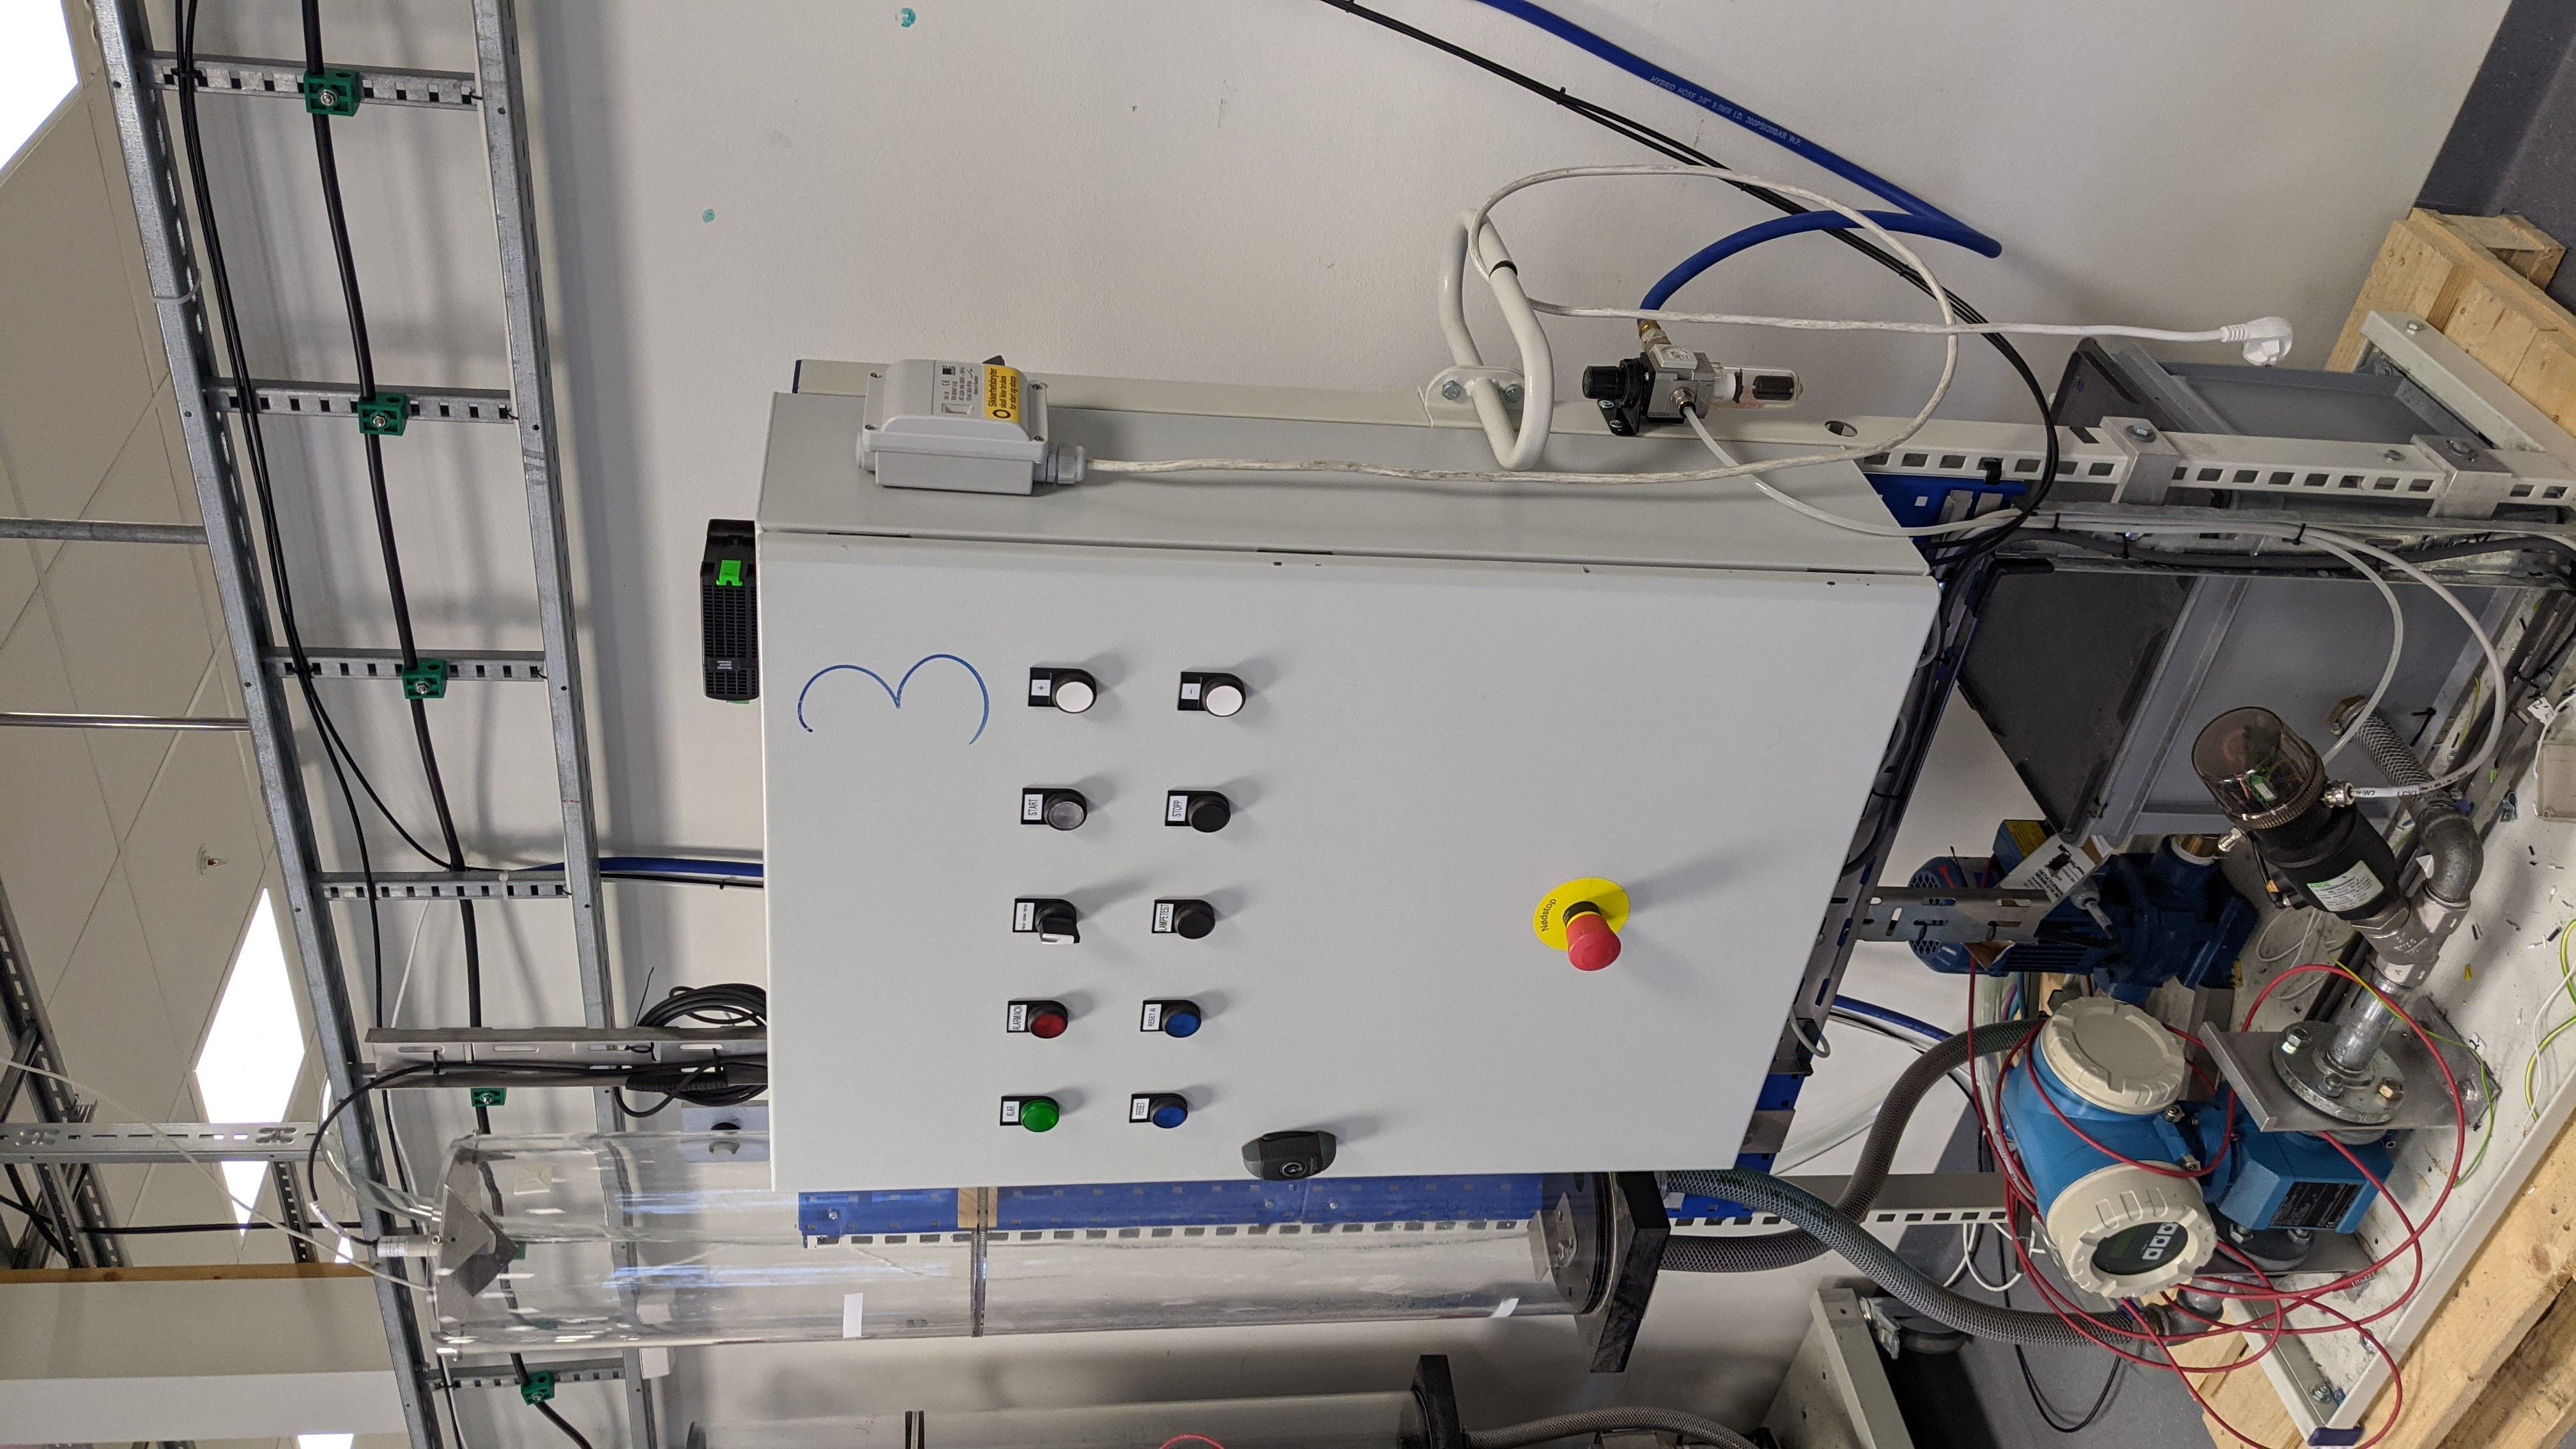
\includegraphics[width=10.5cm,angle=-90]{stasjon03x01.jpg},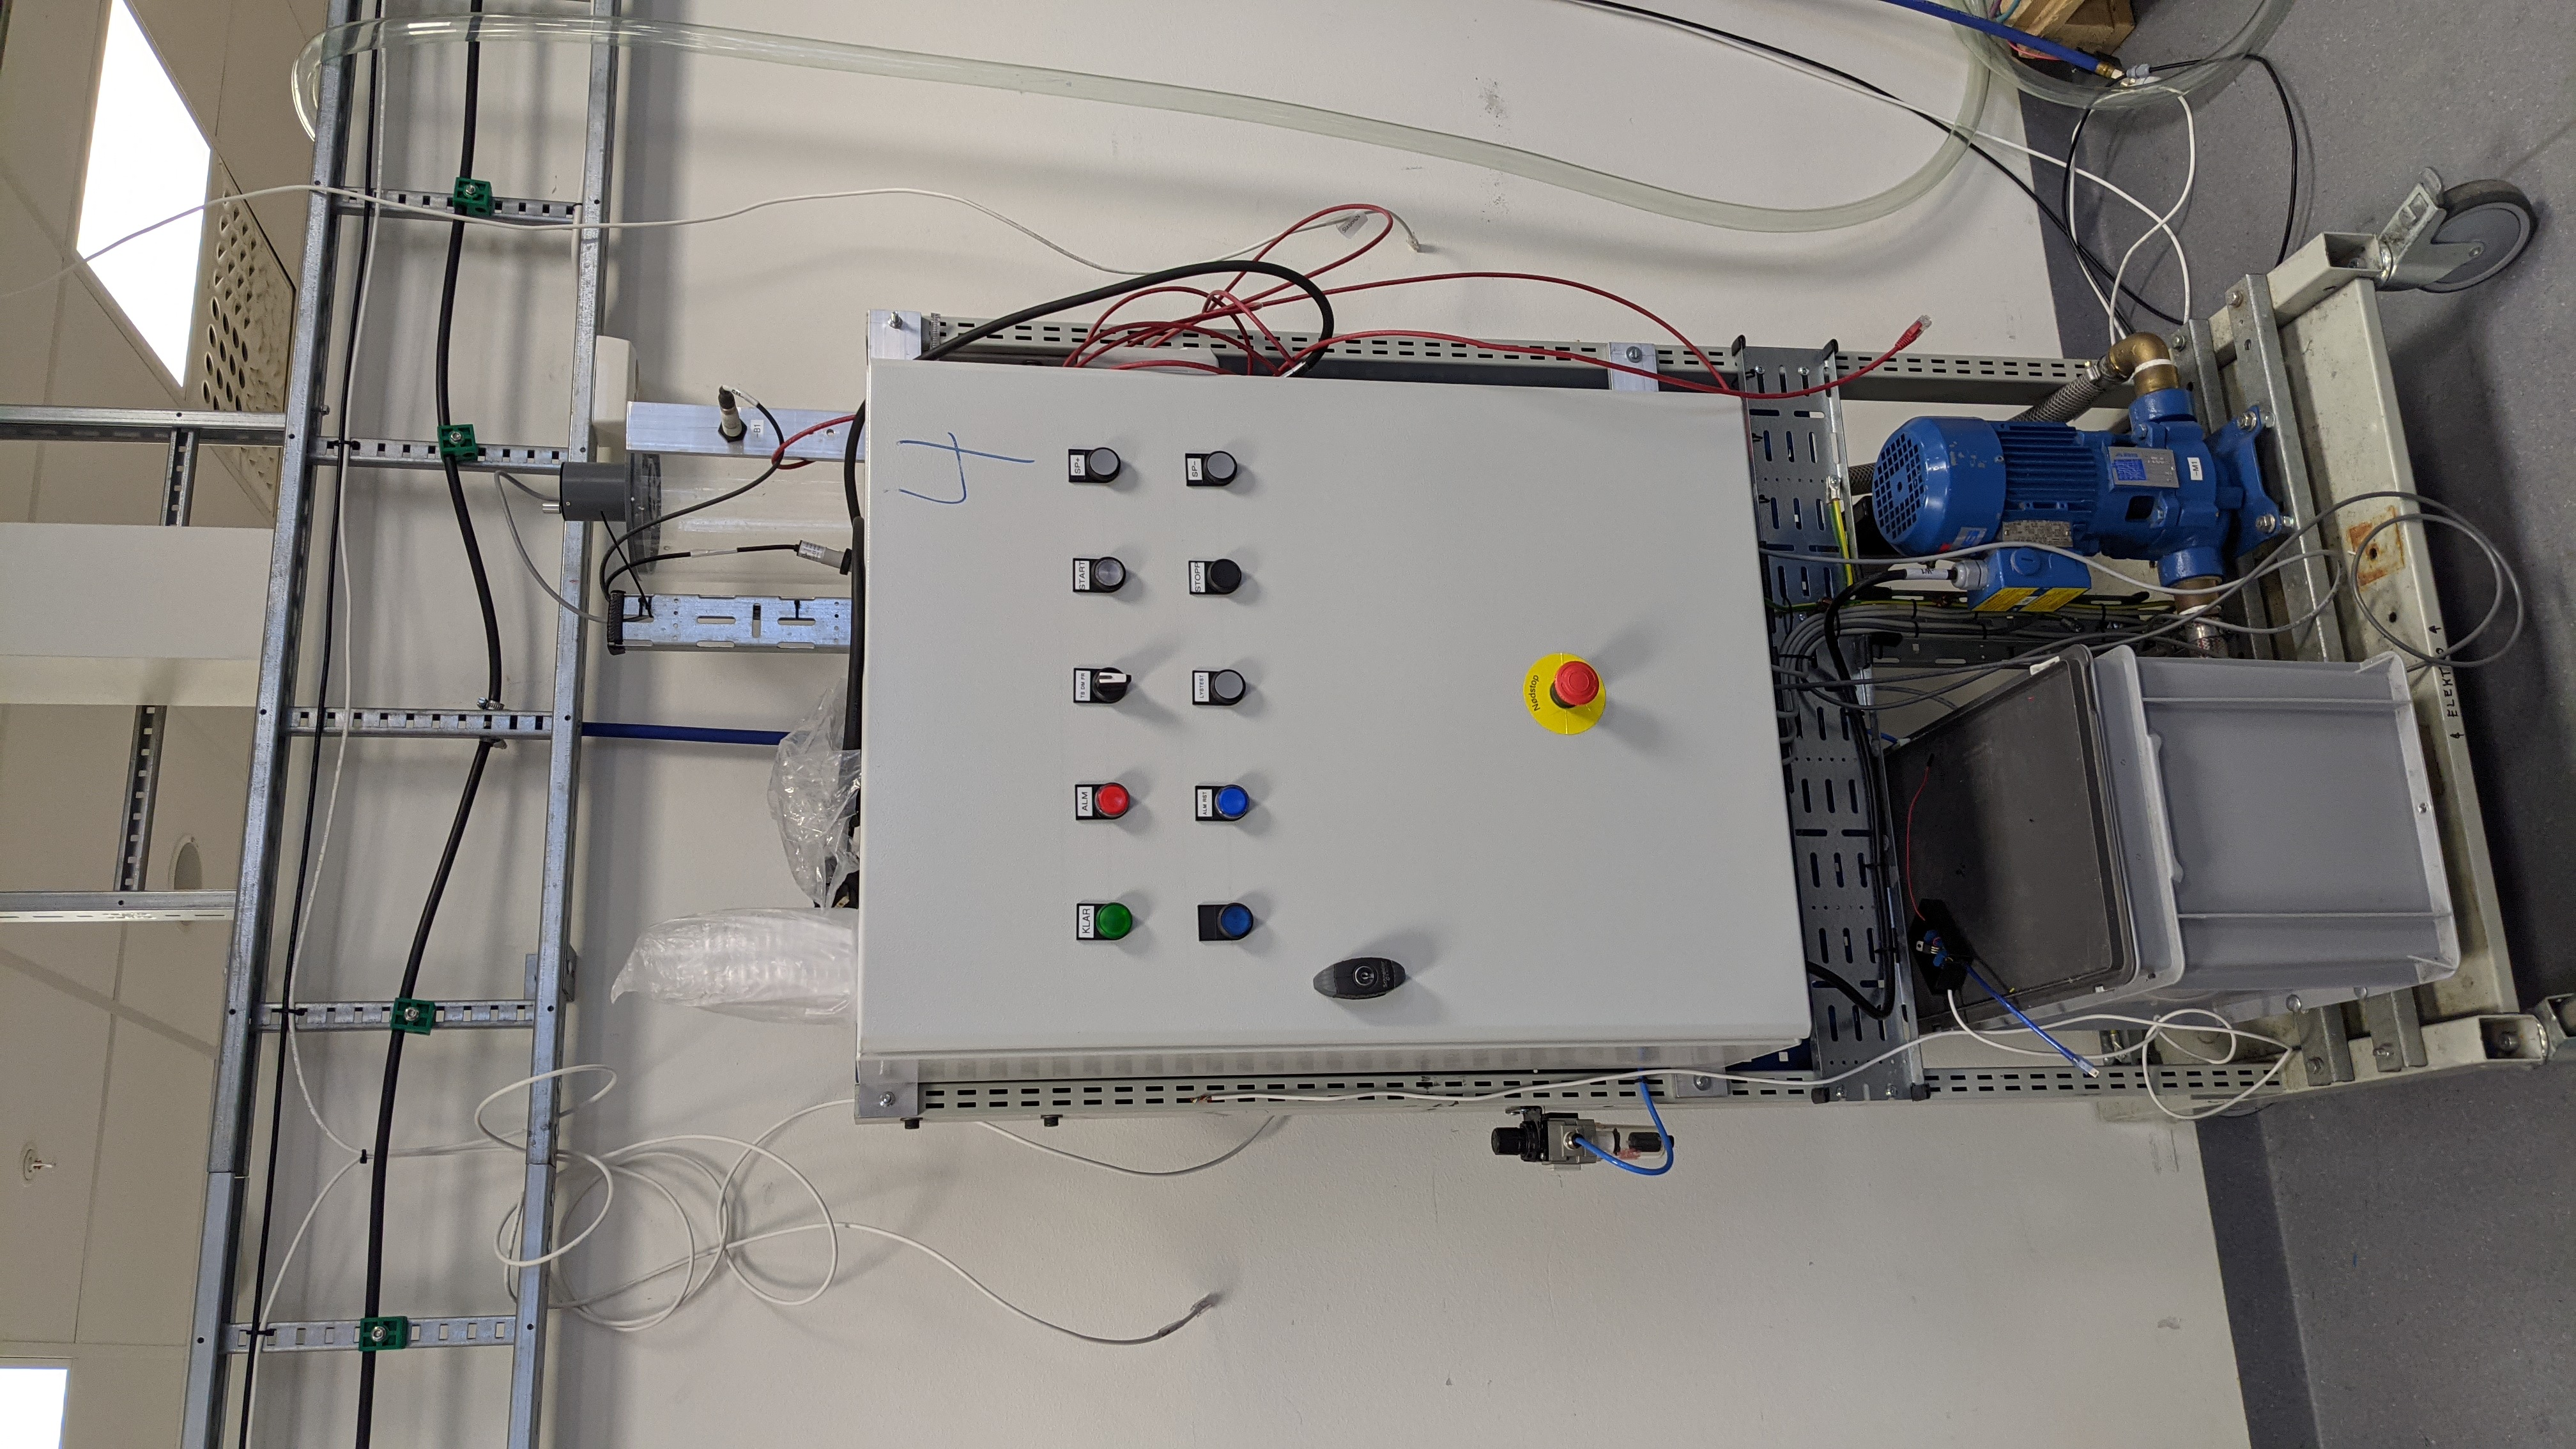
\includegraphics[width=10.5cm,angle=-90]{stasjon04x01.jpg}$$

\newpage


\begin{center}
\textbf{Arbeidsoppdrag på stasjon 04}
\vskip 5pt 
\vskip 5pt 
\end{center}

\vskip 10pt 
\textbf{Introduksjon}

\vskip 5pt 
I dette arbeidsoppdraget skal du gjøre følgende:
\begin{itemize}[noitemsep]
	\item Koble opp stasjonen 
	\item Programmere stasjonen slik at den virker i henhold til spesifikasjon
	\item Lage HMI i henhold til spesifikasjon. 
	\item Optimalisere funksjon og instrumenter. 
\end{itemize}

\textbf{Generelt om stasjon 04}
\vskip 5pt 

Stasjon 04 er en reguleringsmodell, tiltenkt for undervisning i reguleringsteknikk.  

\vskip 5pt 
Stasjonen inneholder to vanntanker koblet sammen med rør, reguleringsventil og pumpe. Det pumpes vann i en tank med nivåmåling. En strømningsmåler måler strøningen ut av tanken. Strømningen ut av tanken styres med en reguleringsventil

\vskip 5pt 
Instrumenteringen på stasjonen består nå av:  
\begin{itemize}[noitemsep]
	\item Gand 01 Ultralyd transmitter
	\item Rosemount 3031 DP-celle
	\item Asco reguleringsventil
	\item Siemens 3~ 230V pumpe
	\item Yaskawa V1000 frekvensomformer
	\item Emerson?? elektromagnetisk strømningsmåler
	\item Wago PFC200 PLS (Codesys runtime)
\end{itemize}

Enkle funksjoner på stasjonen skal kunne styres fra styrepanel på stasjonen. I vanlig bruk skal det være mulig for elever å koble seg opp til stasjonen v.h.a. nettleser og styre den med HMI
\begin{figure}[H]
$$\includegraphics[width=13cm]{lStasjon03x01.eps}$$\\
	\caption {P \& ID over stasjonen}
\end{figure}

\textbf{Generelt om oppgaven}

\vskip 10pt 
Før selve oppgaven påbegynnes skal du utføre en sjekk av utstyret for så å rive ned alle ledninger og kabler. Dere må lage en oversikt over alt utstyr og en plan for å dokumentere at utstyret er i orden. 

I selve arbeidsoppdraget skal du bygge opp, programmere stasjonen, lage et brukergrensesnitt, optimalisere og lage dokumentasjon på stasjonen. 

\vskip 5pt 
 Hovedmomenter i oppgaven vil være: 
\begin{itemize}[noitemsep]
	\item Bygge et styreskap til maskinen
	\item Legge kabel til alt utstyr og implementere dette i styresystemet
	\item Legge opp tilførselskabel til stasjonen, men tilhørende montering av kabelstige 
	\item Programmere styresystem for modellen 
	\item Lage HMI for stasjonen tilpasset opplæring i reguleringsteknikk og koble stasjonen til  nettverk for tilgang til HMI.  
	\item Kalibrering av instrumenter og optimalisering. 
	\item Utarbeiding av dokumentasjon for stasjonen. 
\end{itemize}



 

Design krav:  
\begin{itemize}[noitemsep]
	\item Frekvensomformer skal tilkobles styresystemet v.h.a. feltbuss. 
	\item Det skal brukes sikkerhetsrele til sikkerhetsrelaterte deler av styresystemet
	\item Sikkerhetsrelaterte deler av styresystemet tilkobles frekvensomformeren sin STO funksjon.  
	\item Nivåbryter for høyt nivå i tanken skal tilkobles sikkerhetsrelaterte deler av styresystemet som stopper pumpen med stoppkategori 0.
	\item Det skal være avstenging for all energiforsyning på stasjonen.  
	\item HMI skal i størst mulig grad designes etter prinsippene i «The-High-Performance-HMI-Overview-Part-1-PAS-Inc».  
	\item Enkle funksjoner på stasjonen skal kunne styres fra styrepanel på stasjonen. I vanlig bruk skal det være mulig for elever å koble seg opp til stasjonen v.h.a. nettleser og styre den med HMI.  
	\item dokumentasjon skal være ih.h.t. håndbok for 3AUA
\end{itemize}

\vskip 5pt 
Kompetanser som du skal vise i denne oppgaven:
\begin{itemize}[noitemsep]
	\item Oppkobling av styresystem
	\item Programering av reguleringssystem
	\item Lage HMI for reguleringsstasjon
	\item Dokumentering av automaisert anlegg
	\item Optimalsering av instrumentering
\end{itemize}



\textbf{Stasjonens fuksjonalitet}

\vskip 10pt 

Du skal koble sammen og programmere stajonen slik at den virker på følgende måte:

\vskip 5pt 

Når anlegget spenningsettes må en trykke en resett knapp som aktiverer et grønt «klar» lys. Dette symboliserer at stasjonen er klar til å tas i bruk. Når Sikkerhetsrelaterte deler av styresystemet utløses slukker klar lyset. Når årsaken er utbedret må en igjen trykke resett for å gjøre systemet klart for start.  

\vskip 5pt 
Alarm funksjonalitet: 
\vskip 5pt 
Det skal gis alarm ved følgende tilfeller: 
\begin{itemize}[noitemsep]
\item Ved nivå over 90\% aktiveres en H alarm
\item Ved strømning over 90\% aktiveres en H alarm 

\end{itemize}
\vskip 5pt 
Alarmer skal ha bekreft og reset funksjonalitet. Ved alarm blinker alarm lyset. Når bekreft trykkes lyser det konstant. Når alarm tilstand opphører kan en resette alarmen.  

\vskip 5pt 
Styring av stasjonen gjøres fra HMI i et web grensesnitt.

\vskip 5pt 
Stasjonen skal ha tre funksjonsmodus som velges med en vribryter på fronten:
\begin{itemize}[noitemsep]
	\item Tilbakekoblet regulering med frekvensomformerstyrt pumpe
	\item Kaskadekoblet regulering med ventil (pumpe brukes til å generere forstyrrelser)
	\item Tilbakekoblet regulering av nivå med ventil med konstant pumpetrykk). 
\end{itemize}

\vskip 5pt 
\vskip 5pt 
\textbf{I tilbakekoblet regulering:} 
\begin{itemize}[noitemsep]
	\item Det byttes automatisk til HMI bilde for tilbakekoblet regulering 
	\item Nivå i stasjonen reguleres med ventil.  
	\item Reguleringen startes og stoppes ved hjelp av trykknapper.   
	\item HMI skal vise en forenklet P \& ID av anlegget og gjøre det mulig å optimalisere reguleringen ved hjelp av sprangresponstest på et trace.  
	\item Det skal være et valg for om en ønsker å bruke DP-celle eller ultralydmåler som nivåmåler for reguleringen. Alle nødvendige innstillinger for en reguleringssløyfe skal kunne gjøres fra HMI-en 
	\item Settpunkt skal kunne justeres i hopp på 5\% med + / - knapper på skap.  

\end{itemize}


\textbf{I kaskademodus:}

\begin{itemize}[noitemsep]
	\item Det byttes automatisk til HMI bilde for kaskadekoblet regulering 
	\item Master sløyfen regulerer nivå i tanken. Slavesløyfen regulerer strømning inn i tanken. 
	\item Strømning reguleres med ventilen. 
	\item Pumpen genererer automatiske forstyrrelser for reguleringen. 
	\item Reguleringen startes og stoppes ved hjelp av trykknapper.   
	\item HMI skal vise en forenklet P \& ID av anlegget og gjøre det mulig å optimalisere reguleringen (Master og slave sløyfe) ved hjelp av sprangresponstest på et trace.  
	\item Det skal være et valg for om en ønsker å bruke DP-celle eller ultralydmåler som nivåmåler for reguleringen. Alle nødvendige innstillinger for en reguleringssløyfe skal kunne gjøres fra HMI-en 
	\item Settpunkt skal kunne justeres i hopp på 5\% med + / - knapper på skap.  

\end{itemize}



\textbf{I Foroverkoblet modus:}

\begin{itemize}[noitemsep]
	\item Det byttes automatisk til HMI bilde for konstakt trykk modus 
	\item Pumpen regulerer nivået i tanken, ventilen bruke som forsyrrelse
	\item Strømningsmåling ut av tanken brukes som foroverkobling
	\item Reguleringen startes og stoppes ved hjelp av trykknapper.   
	\item HMI skal vise en forenklet P \& ID av anlegget og gjøre det mulig å optimalisere reguleringene ved hjelp av sprangresponstest på et trace.  
	\item Det skal være et valg for om en ønsker å bruke DP-celle eller ultralydmåler som nivåmåler for reguleringen. Alle nødvendige innstillinger for en reguleringssløyfe skal kunne gjøres fra HMI-en 
	\item Settpunkt skal kunne justeres i hopp på 5\% med + / - knapper på skap.  

\end{itemize}


\href{https://rfka-my.sharepoint.com/:u:/g/personal/fred-olav_mosdal_skole_rogfk_no/EewzybzUnq5PscHy_uJUvUMB3ufsOB417mgUkhGlC8yQrg?e=rPkbpf}{Eksempel program med PID i codesys}

\vskip 5pt 

\vskip 5pt 


 
\vskip 5pt 
\url {https://autofaget.no/pdfs/afgv.pdf}

\end{document}
